\documentclass[12pt]{beamer}

%%%%%%%%%%%%%%%%%%% Theme

\usetheme{metropolis}

%%%%%%%%%%%%%%%%%%% Packages

\usepackage[french, english]{babel}
\usepackage{packages/sleek-beamer}

%%%%%%%%%%%%%%%%%%% Bibliography

\addbibresource{./resources/bib/references.bib}

%%%%%%%%%%%%%%%%%%% Titlepage

\title{Renewable Energy Production Forecast}
\subtitle{PROJ0016 - Big Data Project}
\author{Yann Claes, Gaspard Lambrechts and François Rozet}
\institute{University of Liège}
\date{\today}
\titlelogo{./resources/pdf/logo.pdf}
\framelogo{./resources/pdf/logo.pdf}

%%%%%%%%%%%%%%%%%%%

\DeclareSIUnit\voltampere{VA}

%%%%%%%%%%%%%%%%%%%

\begin{document}

\maketitle

\section{Photovoltaic production}

\begin{frame}{Improvements}
    \begin{itemize}
        \item Maximum power bounding
        \item Temperature influence
        \item Sine scaling
        \item (timezone fixing)
    \end{itemize}
\end{frame}

\begin{frame}{Resulting Model}
    \begin{equation*}
        P_{out} = \min\rbk{\frac{\eta I \cos(\theta) A}{\sin(alt)}, \texttt{MAX\_POW}}
    \end{equation*}
    
    where 
    \begin{equation*}
       \texttt{MAX\_POW} =  \min\rbk{P_{max}, P_{max} - 0.004 (T - 25)}
    \end{equation*}
\end{frame}

\begin{frame}{Updated Model Example}
    Using the thermodynamics laboratory data, the following model is obtained for a period ranging from September 10\up{th} to September 12\up{th}.
\end{frame}

\begin{frame}{Updated Model Example}
    \begin{figure}
        \centering
        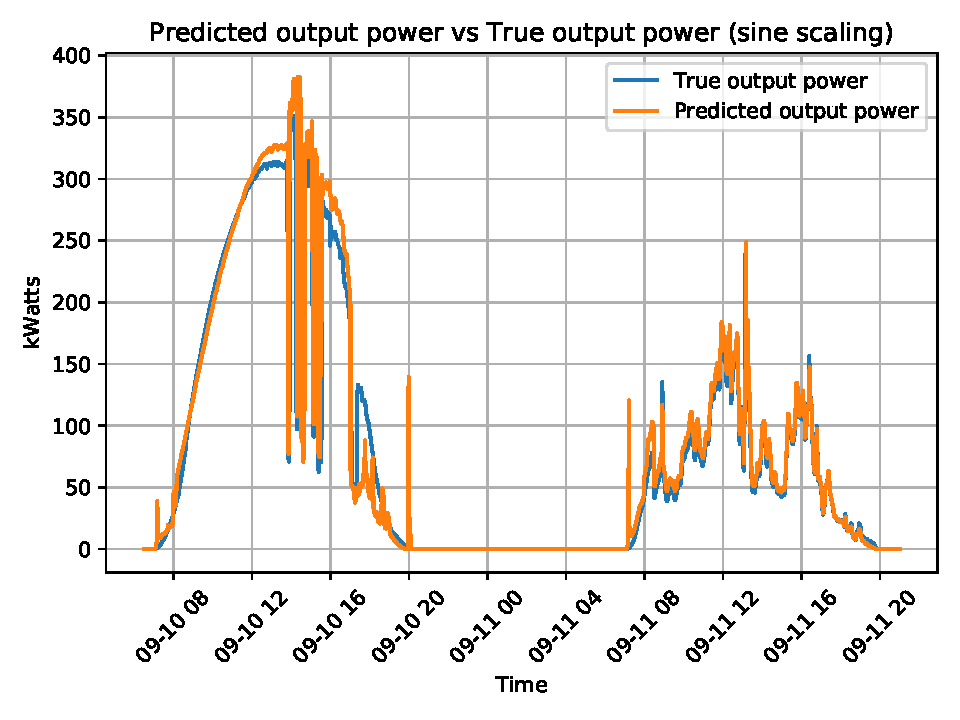
\includegraphics[width=0.9\textwidth]{resources/pdf/predicted_vs_true.pdf}
    \end{figure}
\end{frame}

\begin{frame}{Issue}
    There seems to be peaks at regular periods of the day. By looking at the ratio between the sine and cosine, we notice the existence of peaks as well.
\end{frame}

\begin{frame}{Issue}
    \begin{figure}
        \centering
        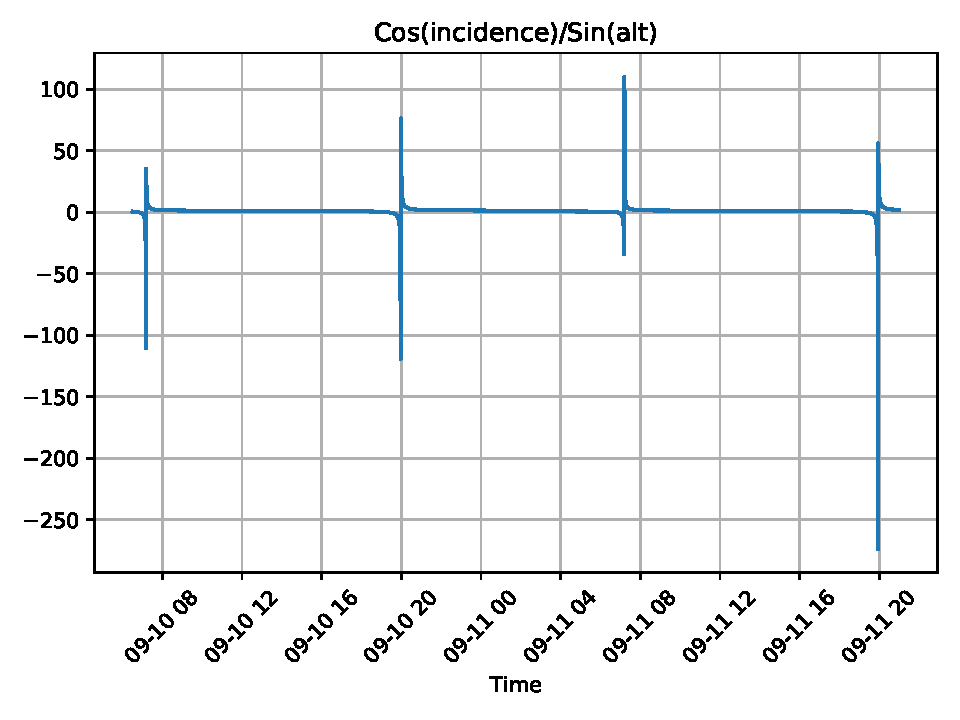
\includegraphics[width=0.9\textwidth]{resources/pdf/cosDIVsin.pdf}
    \end{figure}
\end{frame}

\begin{frame}{Issue}
    To fix the issue, we decided to force the output power to be equal to zero whenever both quantities are negative: it means the sun is \og{}behind\fg{} the panels and has set.
\end{frame}

\begin{frame}{Final model}
    \begin{figure}
        \centering
        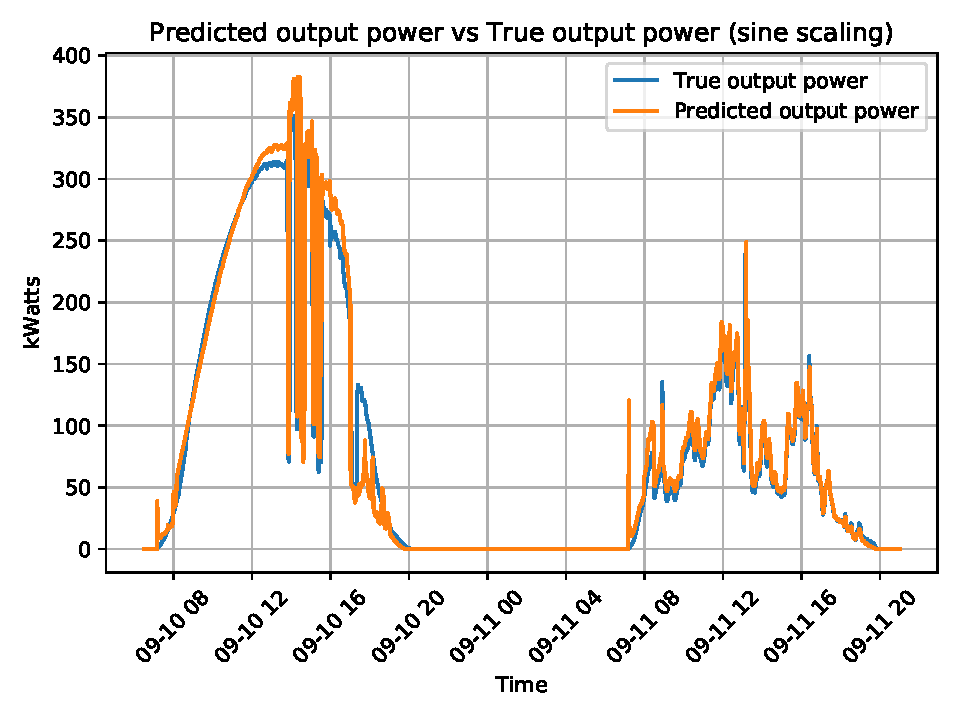
\includegraphics[width=0.9\textwidth]{resources/pdf/final.pdf}
    \end{figure}
\end{frame}

\begin{frame}{Alternative model}
    We have access to old (2017-2018) solar statistics data, containing among others the \si{\kilo\voltampere} (maximum solar power) of photovoltaic panels installed in the municipalities of Liège.
\end{frame}

\begin{frame}{Alternative model}
    Using this, as well as some measure of area of photovoltaic panels per \si{\kilo\watt Peak} ($\sim$ 7), we obtained a rough measure of the average area of photovoltaic panels installed in the province of Liège.
    
    Setting the efficiency $\eta$ to some fixed arbitrary value (\num{0.15}), we obtain the following model (for a period of 3 days).
\end{frame}

\begin{frame}{Alternative model}
    \begin{figure}
        \centering
        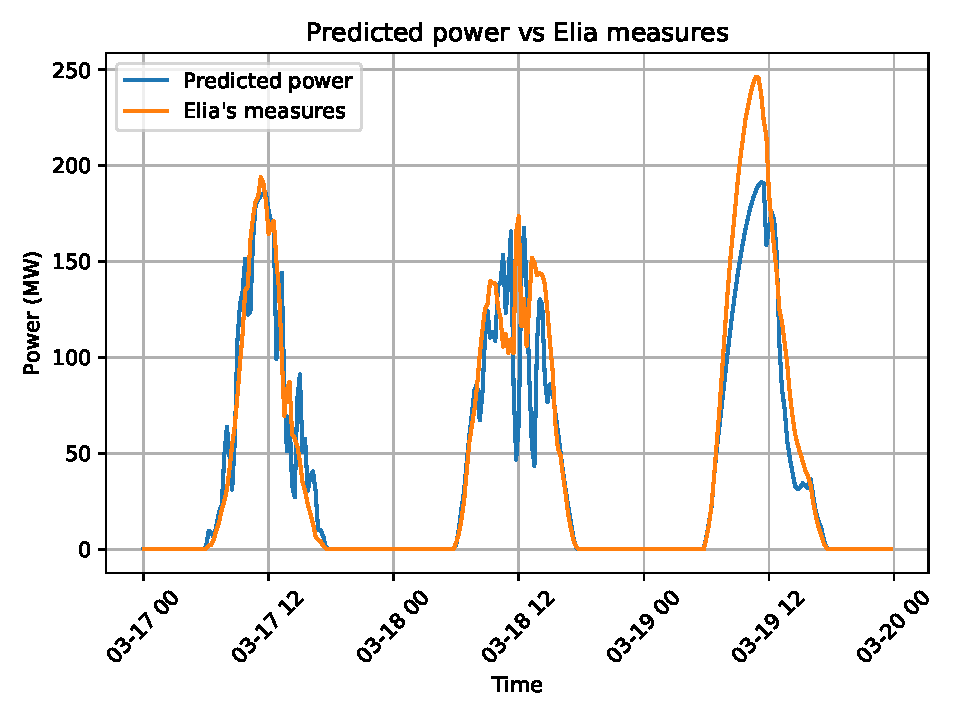
\includegraphics[width=0.9\textwidth]{resources/pdf/province.pdf}
    \end{figure}
\end{frame}

\begin{frame}{Alternative model}
    \begin{itemize}
        \item Use PyStan to fit sensitive parameters to posterior measures made by Elia.
        \item Potentially use Elia's measure of monitored capacity as starting point
    \end{itemize}
\end{frame}

\begin{frame}{Next objectives}
    \begin{itemize}
        \item Deal with uncertainty on parameters ($\eta$, peak area, etc.)
        \item Find relevant irradiance forecast data
    \end{itemize}
\end{frame}

\section{Photovoltaic panels enumeration}

\begin{frame}{Test set -- Google Maps}
    In the previous review, we talked about using the Google Maps satellite imagery for detection (not training) because of its \alert{high resolution}.
    
    Unfortunately, the Google Maps API \alert{isn't} free. Actually, it is probably reserved to commercial use (cannot remove Google watermark).
\end{frame}

\begin{frame}{Test set -- Google Earth Engine}
    Afterwards, we found the \alert{Google Earth Engine} API \cite{earthengine}. It combines a multi-petabyte catalog of satellite imagery and geospatial datasets, like \alert{Landsat} (Nasa) \cite{landsat} and \alert{Sentinel} (Esa) \cite{sentinel}.
    
    The API is primarily available in \alert{JavaScript} and secondarily in \alert{Pyhton}.
    
    The access to this API is restricted, but we obtained the rights.
\end{frame}

\begin{frame}{Test set}
    Unfortunately, the available satellite imagery had an \alert{insufficient resolution} for Belgium.
    
    \alert{WalOnMap} is still our best choice.
\end{frame}

\begin{frame}{Learning set}
    Last review, we proposed a few way to investigate in order to find a learning set.
    
    \begin{itemize}
        \item Asking to a university/repository owner. \visible<3->{We sent multiple mails, \alert{none were answered}.}
        \item OpenStreetMap solar panel coordinates dataset for England. \visible<3->{Gives only (very) approximate location, \alert{not surface nor shape}.}
        \item Keep searching for a dataset. \visible<3->{We found one comming from Duke University ! \cite{figshare}}
    \end{itemize}
\end{frame}

\begin{frame}{Learning set}
    This dataset contains the geospatial coordinates and border vertices for over \alert{\num{19000}} solar panels across \alert{\num{601}} high resolution ($5000 \times 5000$) images from four cities in California (Fresno, Modesto, Oxnard, Stockton).
\end{frame}

\begin{frame}{Learning set}
    \begin{figure}
        \centering
        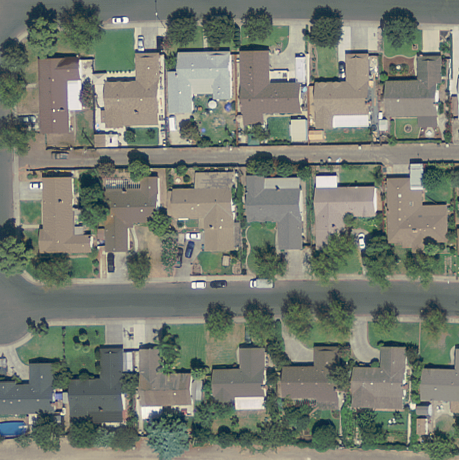
\includegraphics[height=0.8\textheight]{./resources/png/modesto.png}
        \caption{Modesto city, picture 1, zoomed 10 times}
    \end{figure}
\end{frame}

\begin{frame}{Learning set}
    \begin{columns}
        \column{0.4\textwidth}
        The solar panel geospatial coordinates are very precise and provided as \alert{polygon vertices} in either a \alert{\texttt{csv}} or a \alert{\texttt{json}}.
        \column{0.6\textwidth}
        \begin{figure}
            \centering
            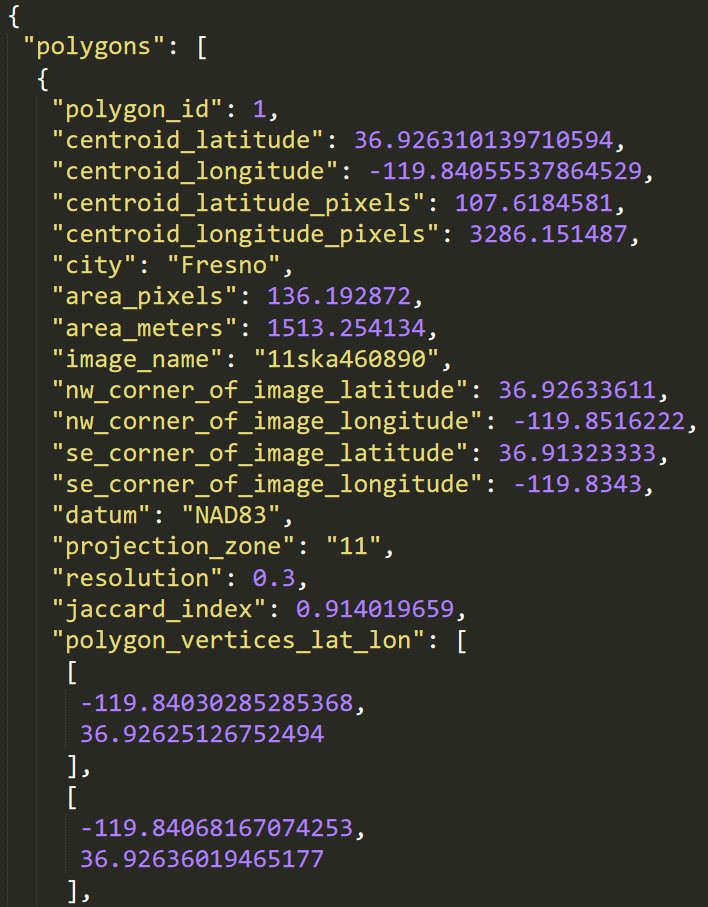
\includegraphics[height=0.8\textheight]{./resources/png/coordinates.png}
            \caption{\texttt{SolarArrayPolygons.json}}
        \end{figure}
    \end{columns}
\end{frame}

\begin{frame}{Learning set}
    These coordinates are not useful \emph{as-is} for training.
    
    We have written (using mainly \alert{\texttt{OpenCV}} \cite{opencv}) a code \texttt{learning\_set.py} to
    \begin{enumerate}
        \item transform the polygons into black and white \alert{classification} images. 
        \item slice the images into smaller ($256 \times 256$) images.
        \item produce $(X, Y)$ image pairs.
    \end{enumerate}
\end{frame}

\begin{frame}{Learning set}
    \begin{figure}
        \centering
        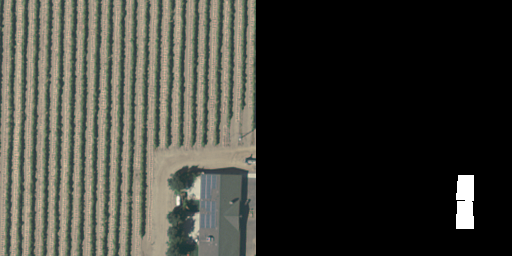
\includegraphics[width=\textwidth]{./resources/png/classification.png}
        \caption{Example of $(X, Y)$ image pair.}
    \end{figure}
\end{frame}

\begin{frame}{Learning set -- Data augmentation}
    We plan to \alert{rotate} and \alert{translate} these $(X, Y)$ image pairs in order to \alert{increase the quantity} of available training data.
\end{frame}

\begin{frame}{Next objectives}
    Now that we have suitable learning and testing sets, we are ready to build our \alert{first detection} model(s).
\end{frame}

\section{Wind production}

\begin{frame}{Data}
New data has been retrieved:
\begin{itemize}
    \item \alert{Wind speed measures} from February 2012 to now (one single location in Wallonia for now)
    \item \alert{Physical model output} using the wind speed measures and the wind turbines data collected for last review, from 2012 to now
    \item Elia's \alert{wind power measures} from February 2012 to now
\end{itemize}
\end{frame}

\begin{frame}{Models}

For now, only four types of models have been investigated.
\begin{itemize}
    \item A \alert{Gaussian Process} based on a Rational Quadratic Kernel predicting the power from the wind speed (at a unique location)
    \item A \alert{Gaussian Process} based on a Rational Quadratic Kernel predicting \alert{residuals} between the measures of Elia and the physical model
    \item A \alert{Random Forest} predicting the power from the wind speed, physical model, and timestamp.
    \item \alert{Extra-Trees} predicting the power from the wind speed, physical model and timestamp.
\end{itemize}

\end{frame}

\begin{frame}{Results - Gaussian Process}
    \begin{figure}
        \centering
        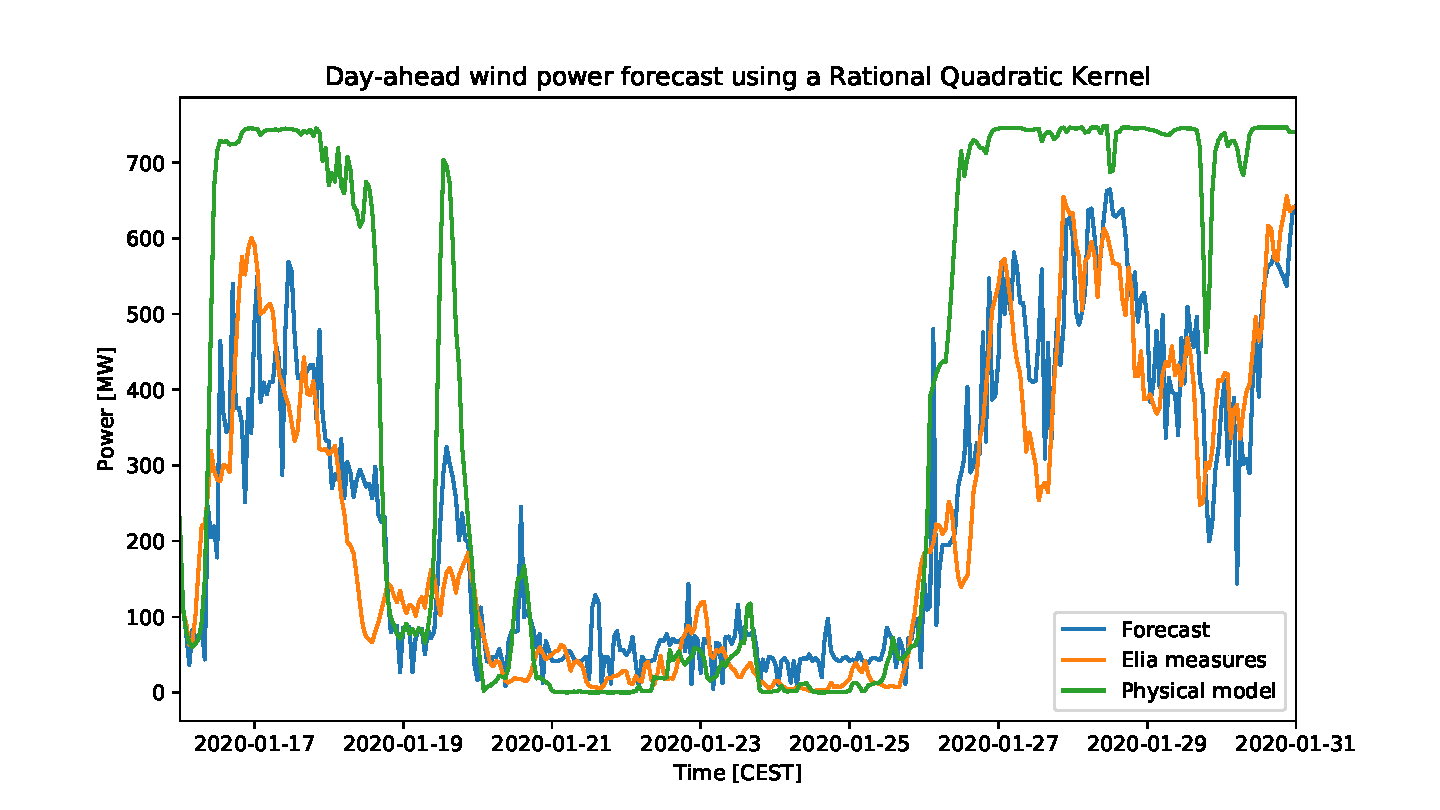
\includegraphics[width=\textwidth]{resources/pdf/dawpf_rqk_1b.pdf}
        \caption{Gaussian Process with Rational Quadratic Kernel - 1 month of training data}
    \end{figure}
\end{frame}

\begin{frame}{Results - Gaussian Process}
    \begin{figure}
        \centering
        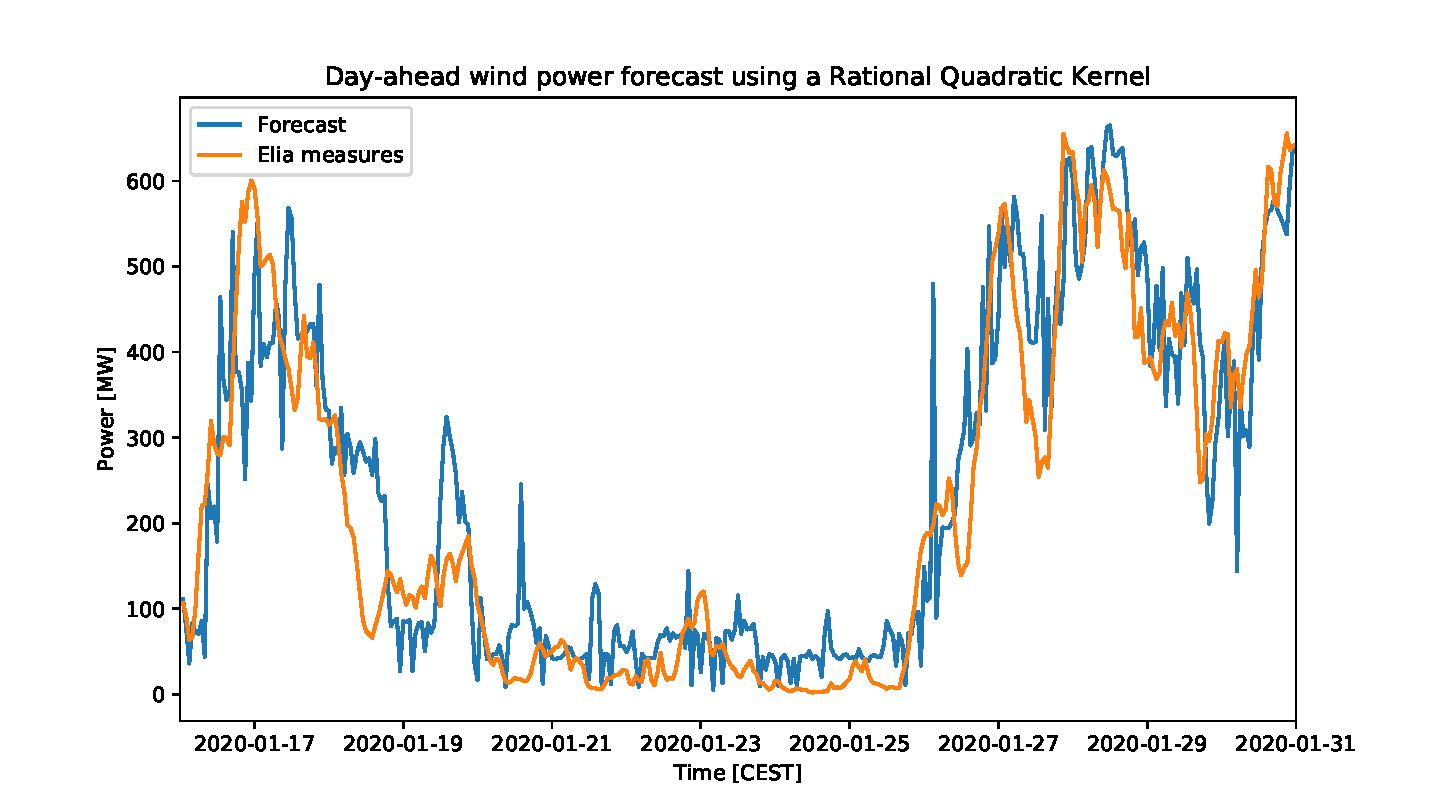
\includegraphics[width=\textwidth]{resources/pdf/dawpf_rqk_1a.pdf}
        \caption{Gaussian Process with Rational Quadratic Kernel - 1 month of training data}
    \end{figure}
\end{frame}

\begin{frame}{Results - Gaussian Process}
    \begin{figure}
        \centering
        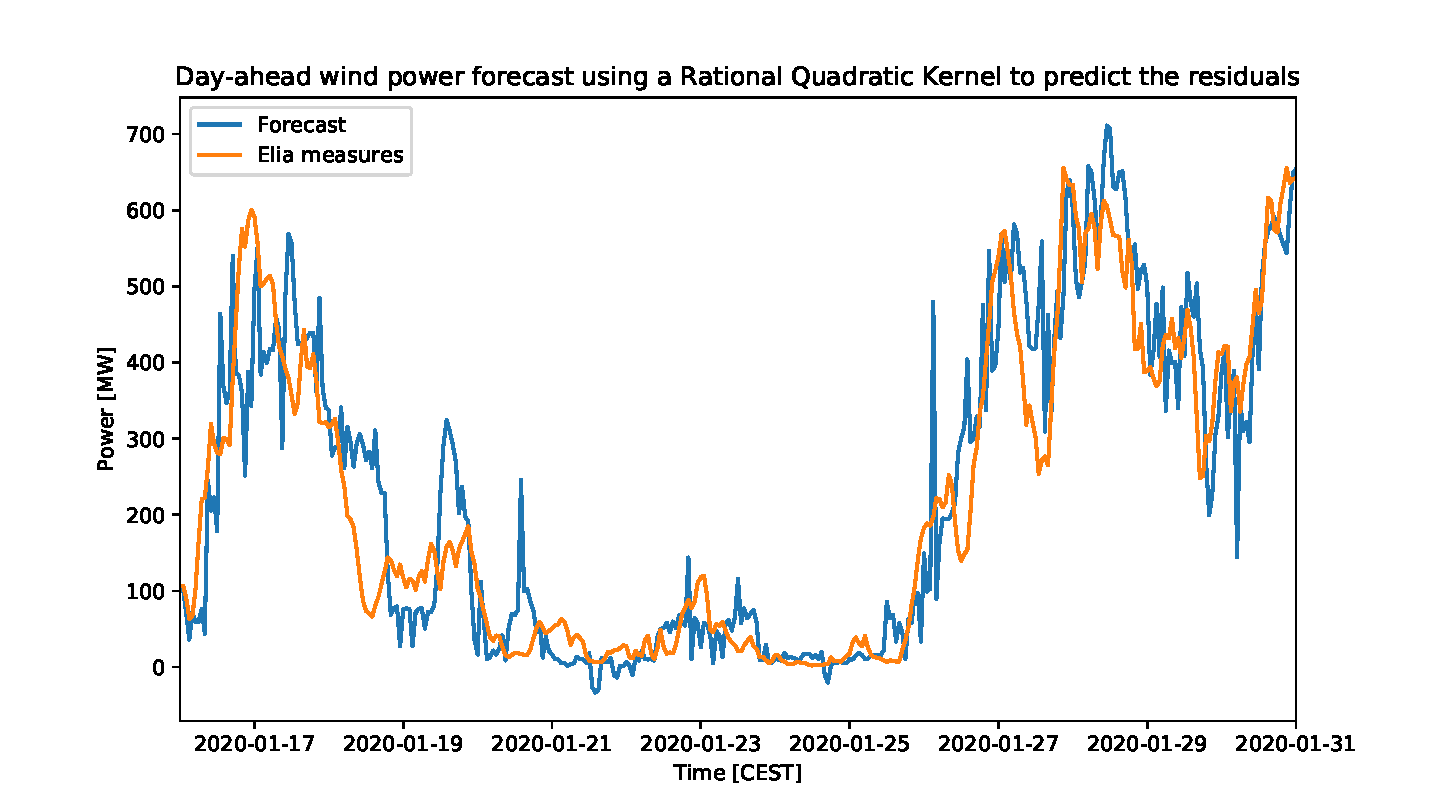
\includegraphics[width=\textwidth]{resources/pdf/dawpf_rqk_r_1a.pdf}
        \caption{Gaussian Process with Rational Quadratic Kernel - 1 month of training data}
    \end{figure}
\end{frame}

\begin{frame}{Results - Gaussian Process}
    \begin{figure}
        \centering
        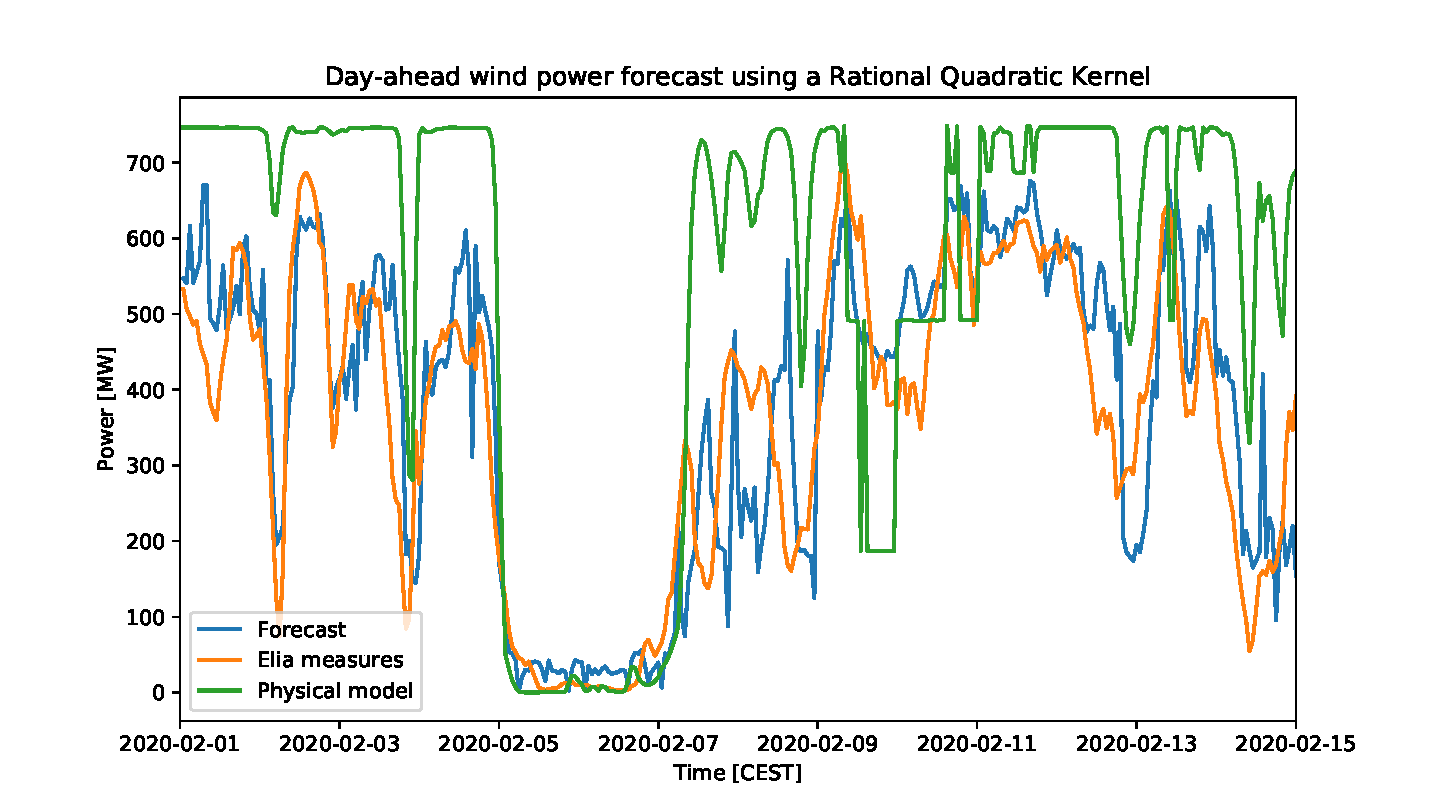
\includegraphics[width=\textwidth]{resources/pdf/dawpf_rqk_2b.pdf}
        \caption{Gaussian Process with Rational Quadratic Kernel - 1 month of training data}
    \end{figure}
\end{frame}

\begin{frame}{Results - Gaussian Process}
    \begin{figure}
        \centering
        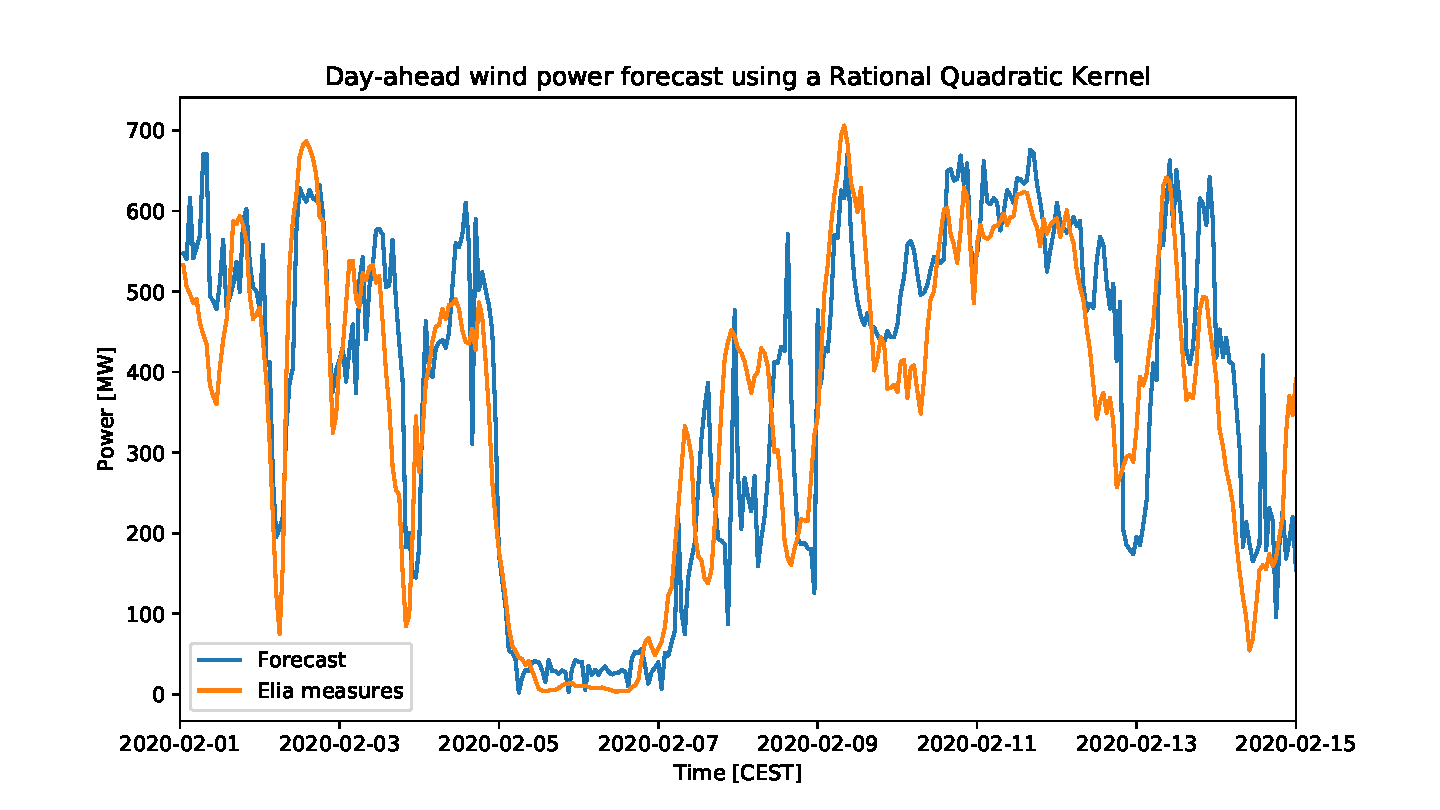
\includegraphics[width=\textwidth]{resources/pdf/dawpf_rqk_2a.pdf}
        \caption{Gaussian Process with Rational Quadratic Kernel - 1 month of training data}
    \end{figure}
\end{frame}

\begin{frame}{Results - Gaussian Process}
    \begin{figure}
        \centering
        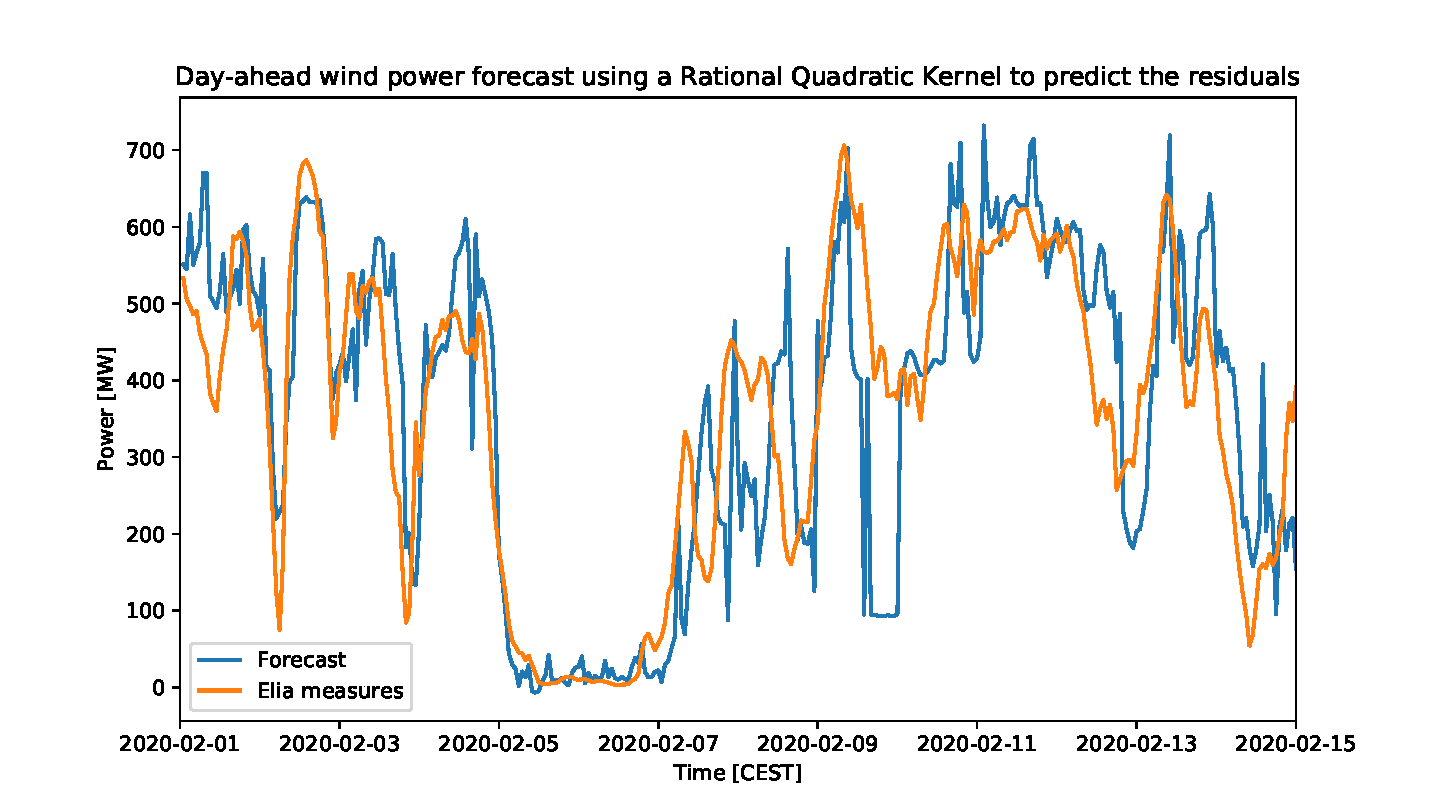
\includegraphics[width=\textwidth]{resources/pdf/dawpf_rqk_r_2a.pdf}
        \caption{Gaussian Process with Rational Quadratic Kernel - 1 month of training data}
    \end{figure}
\end{frame}

\begin{frame}{Results - Gaussian Process - Issues}
    \begin{figure}
        \centering
        \includegraphics[width=\textwidth]{resources/pdf/3.5_months_residuals.pdf}
        \caption{Gaussian Process with Rational Quadratic Kernel - 3 months of training data}
    \end{figure}
\end{frame}

\begin{frame}{Results - Gaussian Process - Issues}
    \begin{figure}
        \centering
        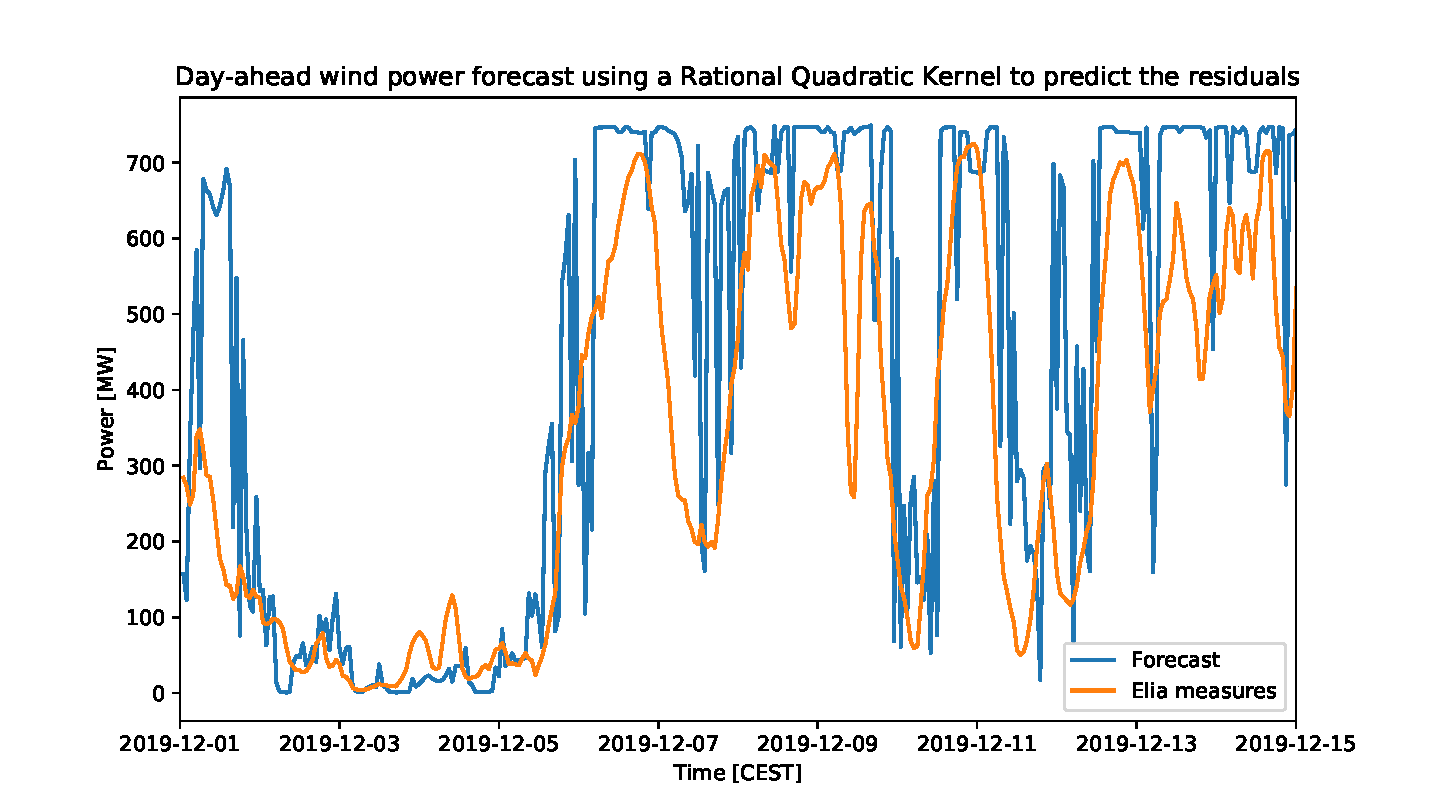
\includegraphics[width=\textwidth]{resources/pdf/idem_sooner_r.pdf}
        \caption{Gaussian Process with Rational Quadratic Kernel - 1 month of training data}
    \end{figure}
\end{frame}

\begin{frame}{Result - Random Forest}
    \begin{figure}
        \centering
        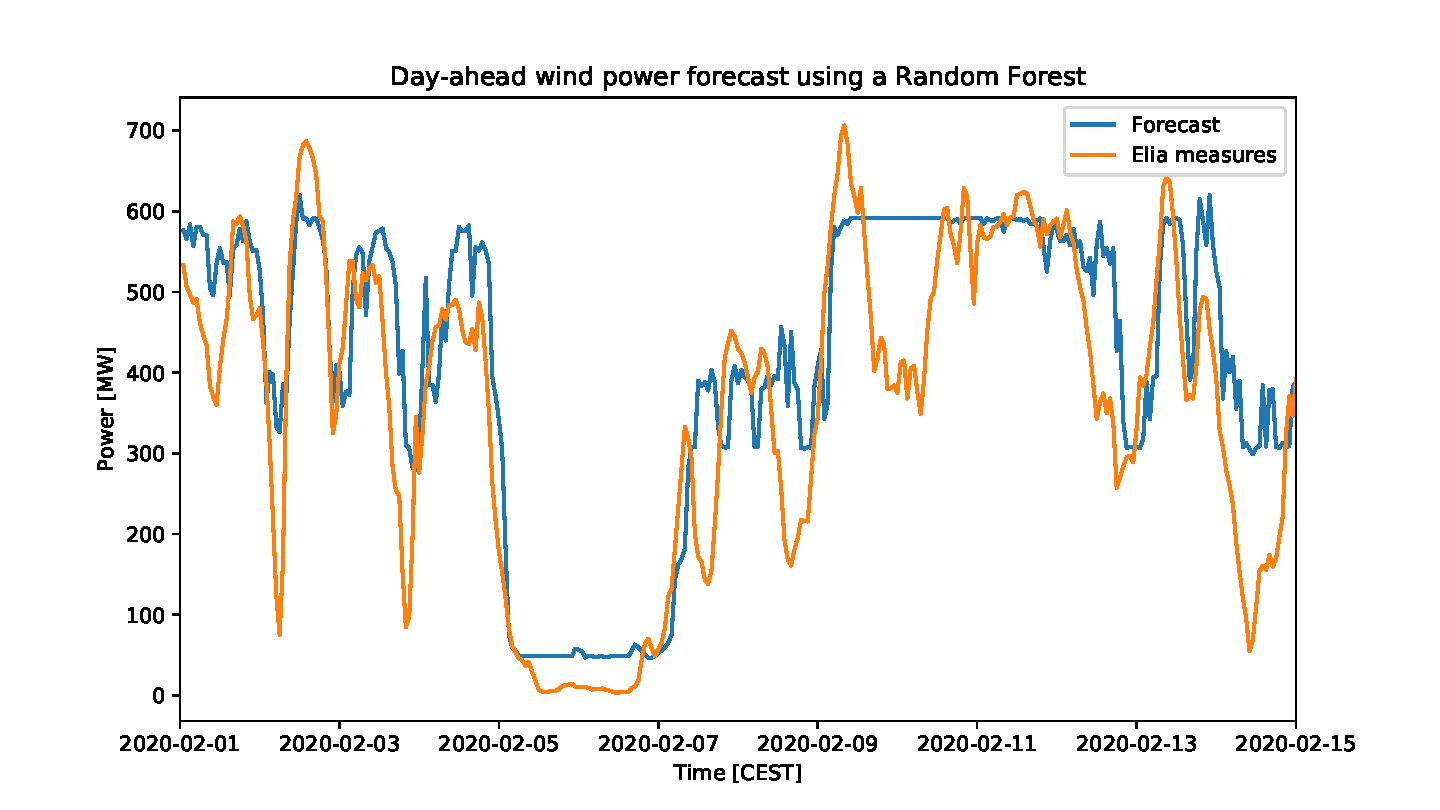
\includegraphics[width=\textwidth]{resources/pdf/rf_one_month.pdf}
        \caption{Random Forest - 1 month of training data}
    \end{figure}
\end{frame}

\begin{frame}{Result - Random Forest}
    \begin{figure}
        \centering
        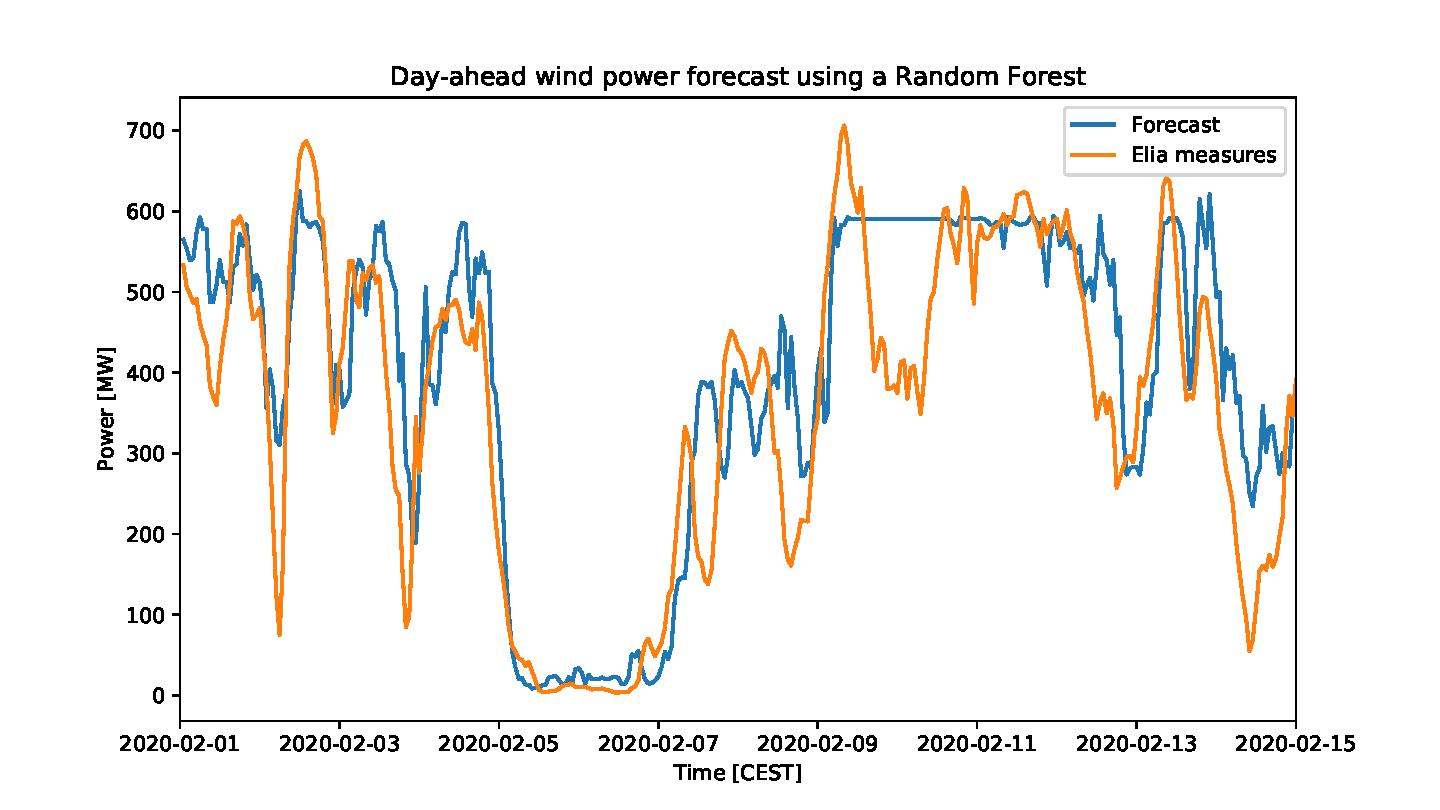
\includegraphics[width=\textwidth]{resources/pdf/rf_one_year.pdf}
        \caption{Random Forest - 1 year of training data}
    \end{figure}
\end{frame}

\begin{frame}{Result - Random Forest}
    \begin{figure}
        \centering
        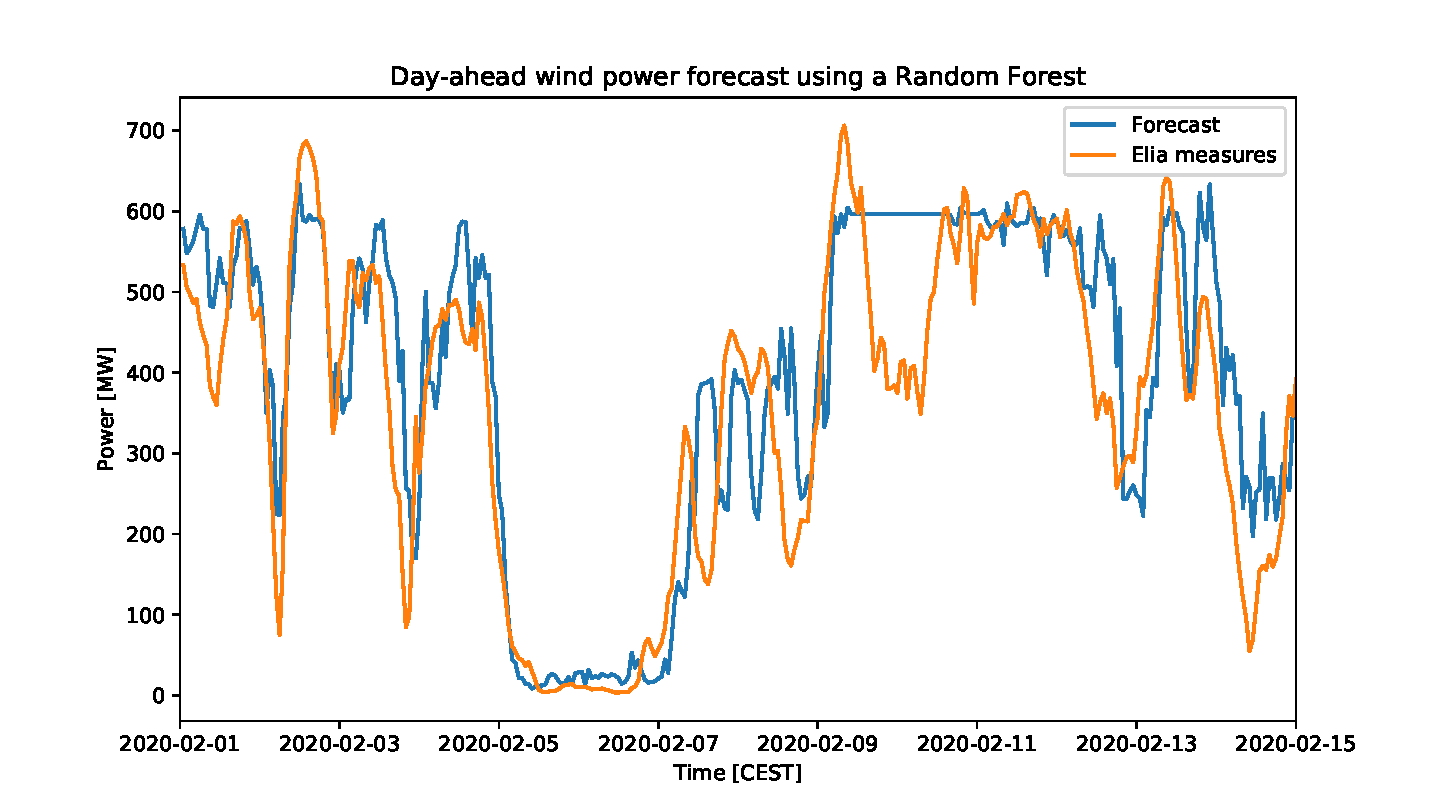
\includegraphics[width=\textwidth]{resources/pdf/rf_8years.pdf}
        \caption{Random Forest - 8 years of training data}
    \end{figure}
\end{frame}

\begin{frame}{Result - Extras Trees}
    \begin{figure}
        \centering
        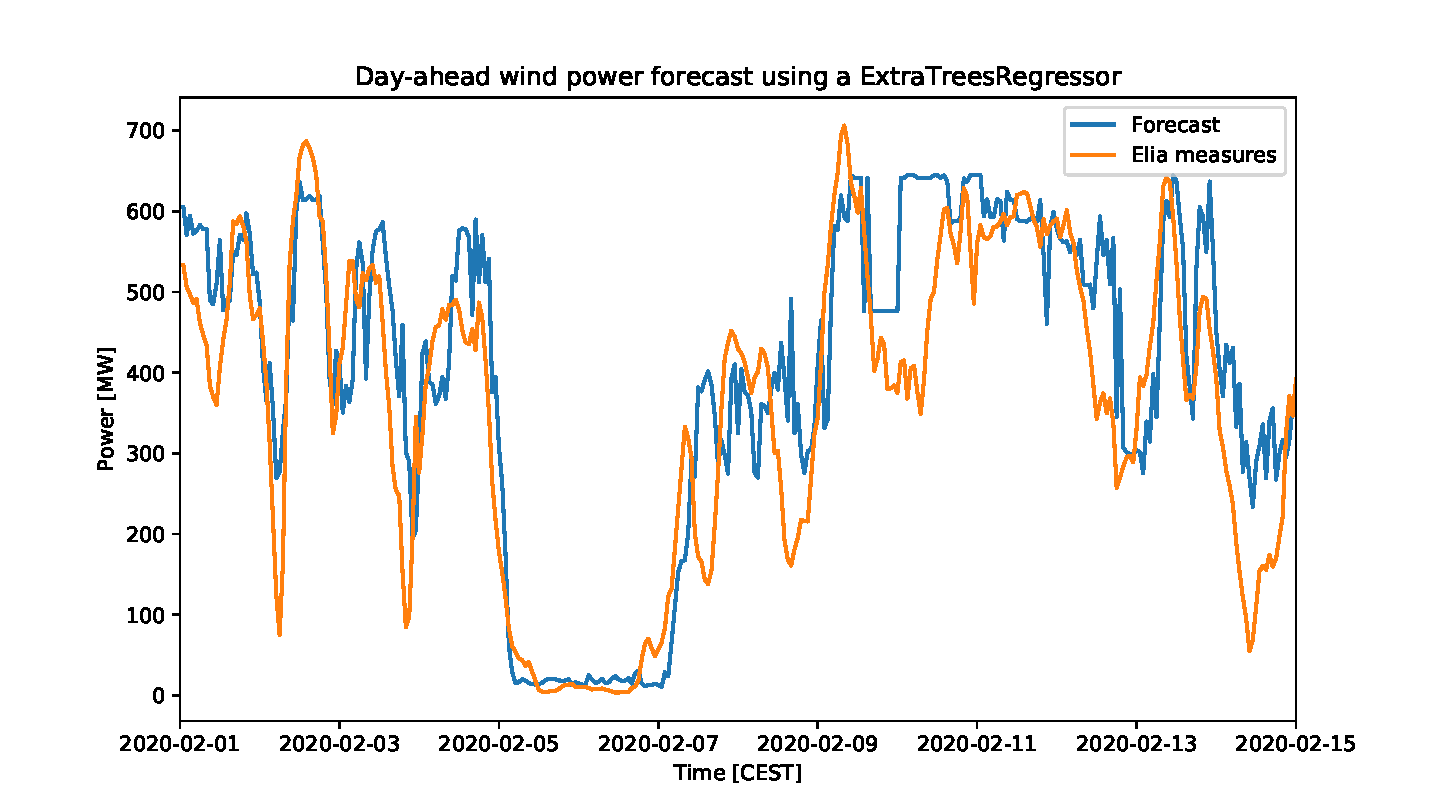
\includegraphics[width=\textwidth]{resources/pdf/xt_1month.pdf}
        \caption{Extra Tree - 1 month of training data}
    \end{figure}
\end{frame}

\begin{frame}{Result - Extras Trees}
    \begin{figure}
        \centering
        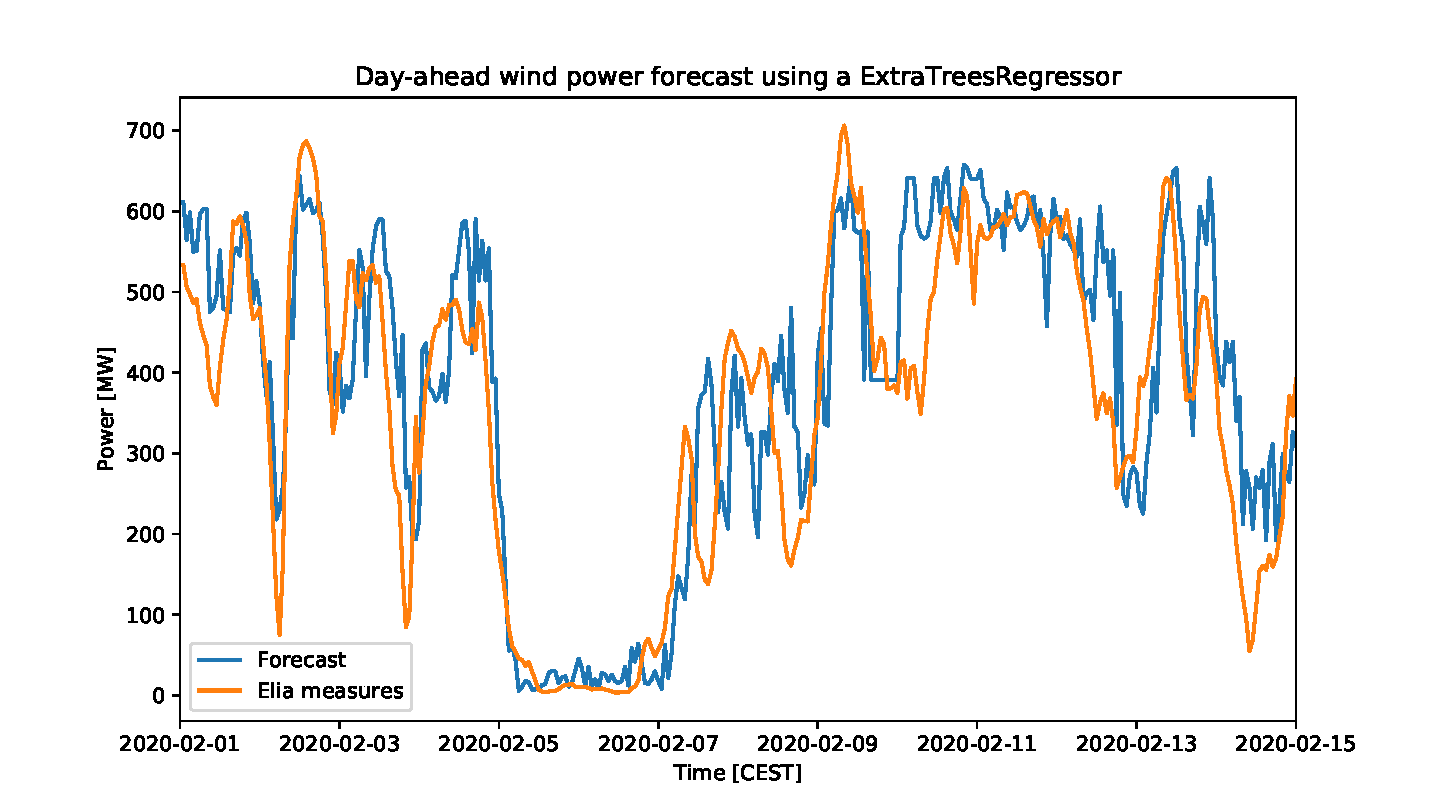
\includegraphics[width=\textwidth]{resources/pdf/xt_one_year.pdf}
        \caption{Extra Tree - 1 year of training data}
    \end{figure}
\end{frame}

\begin{frame}{Result - Extras Trees}
    \begin{figure}
        \centering
        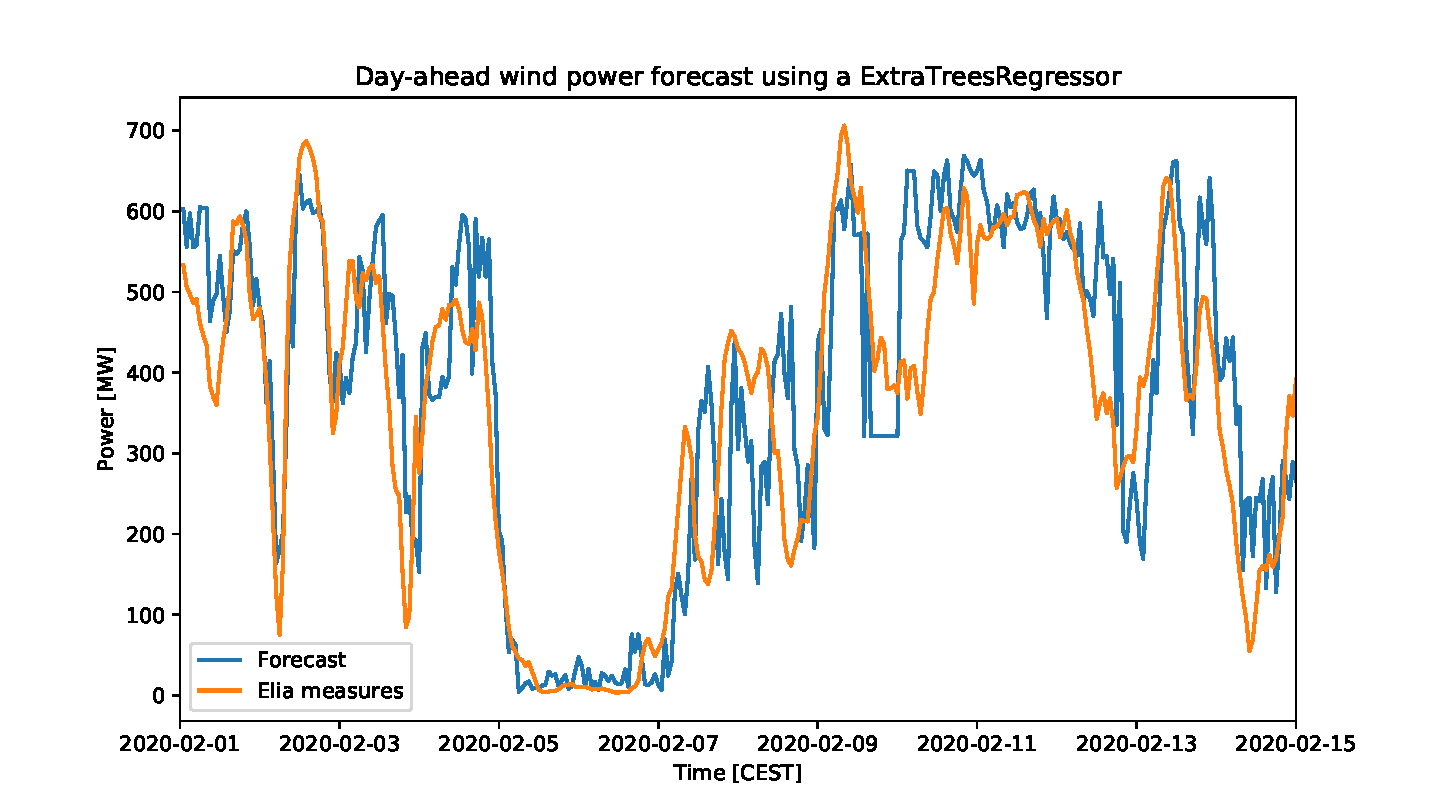
\includegraphics[width=\textwidth]{resources/pdf/xt_8years.pdf}
        \caption{Extra Tree - 8 years of training data}
    \end{figure}
\end{frame}



\begin{frame}[standout]
  Questions ?
\end{frame}

\begin{frame}[allowframebreaks]
    \printbibliography
\end{frame}

\end{document}
